
%% bare_jrnl.tex
%% V1.4
%% 2012/12/27
%% by Michael Shell
%% see http://www.michaelshell.org/
%% for current contact information.
%%
%% This is a skeleton file demonstrating the use of IEEEtran.cls
%% (requires IEEEtran.cls version 1.8 or later) with an IEEE journal paper.
%%
%% Support sites:
%% http://www.michaelshell.org/tex/ieeetran/
%% http://www.ctan.org/tex-archive/macros/latex/contrib/IEEEtran/
%% and
%% http://www.ieee.org/



% *** Authors should verify (and, if needed, correct) their LaTeX system  ***
% *** with the testflow diagnostic prior to trusting their LaTeX platform ***
% *** with production work. IEEE's font choices can trigger bugs that do  ***
% *** not appear when using other class files.                            ***
% The testflow support page is at:
% http://www.michaelshell.org/tex/testflow/


%%*************************************************************************
%% Legal Notice:
%% This code is offered as-is without any warranty either expressed or
%% implied; without even the implied warranty of MERCHANTABILITY or
%% FITNESS FOR A PARTICULAR PURPOSE! 
%% User assumes all risk.
%% In no event shall IEEE or any contributor to this code be liable for
%% any damages or losses, including, but not limited to, incidental,
%% consequential, or any other damages, resulting from the use or misuse
%% of any information contained here.
%%
%% All comments are the opinions of their respective authors and are not
%% necessarily endorsed by the IEEE.
%%
%% This work is distributed under the LaTeX Project Public License (LPPL)
%% ( http://www.latex-project.org/ ) version 1.3, and may be freely used,
%% distributed and modified. A copy of the LPPL, version 1.3, is included
%% in the base LaTeX documentation of all distributions of LaTeX released
%% 2003/12/01 or later.
%% Retain all contribution notices and credits.
%% ** Modified files should be clearly indicated as such, including  **
%% ** renaming them and changing author support contact information. **
%%
%% File list of work: IEEEtran.cls, IEEEtran_HOWTO.pdf, bare_adv.tex,
%%                    bare_conf.tex, bare_jrnl.tex, bare_jrnl_compsoc.tex,
%%                    bare_jrnl_transmag.tex
%%*************************************************************************

% Note that the a4paper option is mainly intended so that authors in
% countries using A4 can easily print to A4 and see how their papers will
% look in print - the typesetting of the document will not typically be
% affected with changes in paper size (but the bottom and side margins will).
% Use the testflow package mentioned above to verify correct handling of
% both paper sizes by the user's LaTeX system.
%
% Also note that the "draftcls" or "draftclsnofoot", not "draft", option
% should be used if it is desired that the figures are to be displayed in
% draft mode.
%
\documentclass[conference]{IEEEtran}
\usepackage[pdftex]{graphicx}
\usepackage{epstopdf}
%
% If IEEEtran.cls has not been installed into the LaTeX system files,
% manually specify the path to it like:
% \documentclass[journal]{../sty/IEEEtran}





% Some very useful LaTeX packages include:
% (uncomment the ones you want to load)


% *** MISC UTILITY PACKAGES ***
%
%\usepackage{ifpdf}
% Heiko Oberdiek's ifpdf.sty is very useful if you need conditional
% compilation based on whether the output is pdf or dvi.
% usage:
% \ifpdf
%   % pdf code
% \else
%   % dvi code
% \fi
% The latest version of ifpdf.sty can be obtained from:
% http://www.ctan.org/tex-archive/macros/latex/contrib/oberdiek/
% Also, note that IEEEtran.cls V1.7 and later provides a builtin
% \ifCLASSINFOpdf conditional that works the same way.
% When switching from latex to pdflatex and vice-versa, the compiler may
% have to be run twice to clear warning/error messages.






% *** CITATION PACKAGES ***
%
\usepackage{cite}
% cite.sty was written by Donald Arseneau
% V1.6 and later of IEEEtran pre-defines the format of the cite.sty package
% \cite{} output to follow that of IEEE. Loading the cite package will
% result in citation numbers being automatically sorted and properly
% "compressed/ranged". e.g., [1], [9], [2], [7], [5], [6] without using
% cite.sty will become [1], [2], [5]--[7], [9] using cite.sty. cite.sty's
% \cite will automatically add leading space, if needed. Use cite.sty's
% noadjust option (cite.sty V3.8 and later) if you want to turn this off
% such as if a citation ever needs to be enclosed in parenthesis.
% cite.sty is already installed on most LaTeX systems. Be sure and use
% version 4.0 (2003-05-27) and later if using hyperref.sty. cite.sty does
% not currently provide for hyperlinked citations.
% The latest version can be obtained at:
% http://www.ctan.org/tex-archive/macros/latex/contrib/cite/
% The documentation is contained in the cite.sty file itself.






% *** GRAPHICS RELATED PACKAGES ***
%
\ifCLASSINFOpdf
   \usepackage[pdftex]{graphicx}
  % declare the path(s) where your graphic files are
   \graphicspath{{../pdf/}{../jpeg/}}
  % and their extensions so you won't have to specify these with
  % every instance of \includegraphics
\DeclareGraphicsExtensions{.pdf,.jpeg,.png}
\else
  % or other class option (dvipsone, dvipdf, if not using dvips). graphicx
  % will default to the driver specified in the system graphics.cfg if no
  % driver is specified.
  % \usepackage[dvips]{graphicx}
  % declare the path(s) where your graphic files are
  % \graphicspath{{../eps/}}
  % and their extensions so you won't have to specify these with
  % every instance of \includegraphics
  % \DeclareGraphicsExtensions{.eps}
\fi
% graphicx was written by David Carlisle and Sebastian Rahtz. It is
% required if you want graphics, photos, etc. graphicx.sty is already
% installed on most LaTeX systems. The latest version and documentation
% can be obtained at: 
% http://www.ctan.org/tex-archive/macros/latex/required/graphics/
% Another good source of documentation is "Using Imported Graphics in
% LaTeX2e" by Keith Reckdahl which can be found at:
% http://www.ctan.org/tex-archive/info/epslatex/
%
% latex, and pdflatex in dvi mode, support graphics in encapsulated
% postscript (.eps) format. pdflatex in pdf mode supports graphics
% in .pdf, .jpeg, .png and .mps (metapost) formats. Users should ensure
% that all non-photo figures use a vector format (.eps, .pdf, .mps) and
% not a bitmapped formats (.jpeg, .png). IEEE frowns on bitmapped formats
% which can result in "jaggedy"/blurry rendering of lines and letters as
% well as large increases in file sizes.
%
% You can find documentation about the pdfTeX application at:
% http://www.tug.org/applications/pdftex





% *** MATH PACKAGES ***
%
\usepackage[cmex10]{amsmath}
% A popular package from the American Mathematical Society that provides
% many useful and powerful commands for dealing with mathematics. If using
% it, be sure to load this package with the cmex10 option to ensure that
% only type 1 fonts will utilized at all point sizes. Without this option,
% it is possible that some math symbols, particularly those within
% footnotes, will be rendered in bitmap form which will result in a
% document that can not be IEEE Xplore compliant!
%
% Also, note that the amsmath package sets \interdisplaylinepenalty to 10000
% thus preventing page breaks from occurring within multiline equations. Use:
\interdisplaylinepenalty=2500
% after loading amsmath to restore such page breaks as IEEEtran.cls normally
% does. amsmath.sty is already installed on most LaTeX systems. The latest
% version and documentation can be obtained at:
% http://www.ctan.org/tex-archive/macros/latex/required/amslatex/math/





% *** SPECIALIZED LIST PACKAGES ***
%
%\usepackage{algorithmic}
% algorithmic.sty was written by Peter Williams and Rogerio Brito.
% This package provides an algorithmic environment fo describing algorithms.
% You can use the algorithmic environment in-text or within a figure
% environment to provide for a floating algorithm. Do NOT use the algorithm
% floating environment provided by algorithm.sty (by the same authors) or
% algorithm2e.sty (by Christophe Fiorio) as IEEE does not use dedicated
% algorithm float types and packages that provide these will not provide
% correct IEEE style captions. The latest version and documentation of
% algorithmic.sty can be obtained at:
% http://www.ctan.org/tex-archive/macros/latex/contrib/algorithms/
% There is also a support site at:
% http://algorithms.berlios.de/index.html
% Also of interest may be the (relatively newer and more customizable)
% algorithmicx.sty package by Szasz Janos:
% http://www.ctan.org/tex-archive/macros/latex/contrib/algorithmicx/




% *** ALIGNMENT PACKAGES ***
%
\usepackage{array}
% Frank Mittelbach's and David Carlisle's array.sty patches and improves
% the standard LaTeX2e array and tabular environments to provide better
% appearance and additional user controls. As the default LaTeX2e table
% generation code is lacking to the point of almost being broken with
% respect to the quality of the end results, all users are strongly
% advised to use an enhanced (at the very least that provided by array.sty)
% set of table tools. array.sty is already installed on most systems. The
% latest version and documentation can be obtained at:
% http://www.ctan.org/tex-archive/macros/latex/required/tools/


% IEEEtran contains the IEEEeqnarray family of commands that can be used to
% generate multiline equations as well as matrices, tables, etc., of high
% quality.




% *** SUBFIGURE PACKAGES ***
%\ifCLASSOPTIONcompsoc
%  \usepackage[caption=false,font=normalsize,labelfont=sf,textfont=sf]{subfig}
%\else
%  \usepackage[caption=false,font=footnotesize]{subfig}
%\fi
% subfig.sty, written by Steven Douglas Cochran, is the modern replacement
% for subfigure.sty, the latter of which is no longer maintained and is
% incompatible with some LaTeX packages including fixltx2e. However,
% subfig.sty requires and automatically loads Axel Sommerfeldt's caption.sty
% which will override IEEEtran.cls' handling of captions and this will result
% in non-IEEE style figure/table captions. To prevent this problem, be sure
% and invoke subfig.sty's "caption=false" package option (available since
% subfig.sty version 1.3, 2005/06/28) as this is will preserve IEEEtran.cls
% handling of captions.
% Note that the Computer Society format requires a larger sans serif font
% than the serif footnote size font used in traditional IEEE formatting
% and thus the need to invoke different subfig.sty package options depending
% on whether compsoc mode has been enabled.
%
% The latest version and documentation of subfig.sty can be obtained at:
% http://www.ctan.org/tex-archive/macros/latex/contrib/subfig/




% *** FLOAT PACKAGES ***
%
%\usepackage{fixltx2e}
% fixltx2e, the successor to the earlier fix2col.sty, was written by
% Frank Mittelbach and David Carlisle. This package corrects a few problems
% in the LaTeX2e kernel, the most notable of which is that in current
% LaTeX2e releases, the ordering of single and double column floats is not
% guaranteed to be preserved. Thus, an unpatched LaTeX2e can allow a
% single column figure to be placed prior to an earlier double column
% figure. The latest version and documentation can be found at:
% http://www.ctan.org/tex-archive/macros/latex/base/

\usepackage{threeparttable}

%\usepackage{stfloats}
% stfloats.sty was written by Sigitas Tolusis. This package gives LaTeX2e
% the ability to do double column floats at the bottom of the page as well
% as the top. (e.g., "\begin{figure*}[!b]" is not normally possible in
% LaTeX2e). It also provides a command:
%\fnbelowfloat
% to enable the placement of footnotes below bottom floats (the standard
% LaTeX2e kernel puts them above bottom floats). This is an invasive package
% which rewrites many portions of the LaTeX2e float routines. It may not work
% with other packages that modify the LaTeX2e float routines. The latest
% version and documentation can be obtained at:
% http://www.ctan.org/tex-archive/macros/latex/contrib/sttools/
% Do not use the stfloats baselinefloat ability as IEEE does not allow
% \baselineskip to stretch. Authors submitting work to the IEEE should note
% that IEEE rarely uses double column equations and that authors should try
% to avoid such use. Do not be tempted to use the cuted.sty or midfloat.sty
% packages (also by Sigitas Tolusis) as IEEE does not format its papers in
% such ways.
% Do not attempt to use stfloats with fixltx2e as they are incompatible.
% Instead, use Morten Hogholm'a dblfloatfix which combines the features
% of both fixltx2e and stfloats:
%
% \usepackage{dblfloatfix}
% The latest version can be found at:
% http://www.ctan.org/tex-archive/macros/latex/contrib/dblfloatfix/




%\ifCLASSOPTIONcaptionsoff
%  \usepackage[nomarkers]{endfloat}
% \let\MYoriglatexcaption\caption
% \renewcommand{\caption}[2][\relax]{\MYoriglatexcaption[#2]{#2}}
%\fi
% endfloat.sty was written by James Darrell McCauley, Jeff Goldberg and 
% Axel Sommerfeldt. This package may be useful when used in conjunction with 
% IEEEtran.cls'  captionsoff option. Some IEEE journals/societies require that
% submissions have lists of figures/tables at the end of the paper and that
% figures/tables without any captions are placed on a page by themselves at
% the end of the document. If needed, the draftcls IEEEtran class option or
% \CLASSINPUTbaselinestretch interface can be used to increase the line
% spacing as well. Be sure and use the nomarkers option of endfloat to
% prevent endfloat from "marking" where the figures would have been placed
% in the text. The two hack lines of code above are a slight modification of
% that suggested by in the endfloat docs (section 8.4.1) to ensure that
% the full captions always appear in the list of figures/tables - even if
% the user used the short optional argument of \caption[]{}.
% IEEE papers do not typically make use of \caption[]'s optional argument,
% so this should not be an issue. A similar trick can be used to disable
% captions of packages such as subfig.sty that lack options to turn off
% the subcaptions:
% For subfig.sty:
% \let\MYorigsubfloat\subfloat
% \renewcommand{\subfloat}[2][\relax]{\MYorigsubfloat[]{#2}}
% However, the above trick will not work if both optional arguments of
% the \subfloat command are used. Furthermore, there needs to be a
% description of each subfigure *somewhere* and endfloat does not add
% subfigure captions to its list of figures. Thus, the best approach is to
% avoid the use of subfigure captions (many IEEE journals avoid them anyway)
% and instead reference/explain all the subfigures within the main caption.
% The latest version of endfloat.sty and its documentation can obtained at:
% http://www.ctan.org/tex-archive/macros/latex/contrib/endfloat/
%
% The IEEEtran \ifCLASSOPTIONcaptionsoff conditional can also be used
% later in the document, say, to conditionally put the References on a 
% page by themselves.




% *** PDF, URL AND HYPERLINK PACKAGES ***
%
%\usepackage{url}
% url.sty was written by Donald Arseneau. It provides better support for
% handling and breaking URLs. url.sty is already installed on most LaTeX
% systems. The latest version and documentation can be obtained at:
% http://www.ctan.org/tex-archive/macros/latex/contrib/url/
% Basically, \url{my_url_here}.




% *** Do not adjust lengths that control margins, column widths, etc. ***
% *** Do not use packages that alter fonts (such as pslatex).         ***
% There should be no need to do such things with IEEEtran.cls V1.6 and later.
% (Unless specifically asked to do so by the journal or conference you plan
% to submit to, of course. )


% correct bad hyphenation here
\hyphenation{op-tical net-works semi-conduc-tor}


\begin{document}
%
% paper title
% can use linebreaks \\ within to get better formatting as desired
% Do not put math or special symbols in the title.
\title{A Restricted Boltzmann Machine Based Two-lead Electrocardiography Classification}
%
%
% author names and IEEE memberships
% note positions of commas and nonbreaking spaces ( ~ ) LaTeX will not break
% a structure at a ~ so this keeps an author's name from being broken across
% two lines.
% use \thanks{} to gain access to the first footnote area
% a separate \thanks must be used for each paragraph as LaTeX2e's \thanks
% was not built to handle multiple paragraphs
%


\author{\IEEEauthorblockN{Yan Yan}
\IEEEauthorblockA{Shenzhen Institutes of Advanced \\
Technology, Chinese \\
Academy of Sciences\\
Email: yan.yan@siat.ac.cn}
\and
\IEEEauthorblockN{Xinbing Qin}
\IEEEauthorblockA{Shenzhen Institutes of Advanced \\
Technology, Chinese \\
Academy of Sciences\\
Email: xb.qin@siat.ac.cn}
\and
\IEEEauthorblockN{Jianping Fan\\ and Lei Wang}
\IEEEauthorblockA{Shenzhen Institutes of Advanced\\ 
Technology, Chinese \\
Academy of Sciences\\}}

% note the % following the last \IEEEmembership and also \thanks - 
% these prevent an unwanted space from occurring between the last author name
% and the end of the author line. i.e., if you had this:
% 
% \author{....lastname \thanks{...} \thanks{...} }
%                     ^------------^------------^----Do not want these spaces!
%
% a space would be appended to the last name and could cause every name on that
% line to be shifted left slightly. This is one of those "LaTeX things". For
% instance, "\textbf{A} \textbf{B}" will typeset as "A B" not "AB". To get
% "AB" then you have to do: "\textbf{A}\textbf{B}"
% \thanks is no different in this regard, so shield the last } of each \thanks
% that ends a line with a % and do not let a space in before the next \thanks.
% Spaces after \IEEEmembership other than the last one are OK (and needed) as
% you are supposed to have spaces between the names. For what it is worth,
% this is a minor point as most people would not even notice if the said evil
% space somehow managed to creep in.




% make the title area
\maketitle

% As a general rule, do not put math, special symbols or citations
% in the abstract or keywords.
\begin{abstract}
An restricted Boltzmann machine learning algorithm were proposed in the two-lead heart beat classification problem.
ECG classification is a complex pattern recognition problem. The unsupervised learning algorithm of restricted Boltzmann machine is ideal in mining the massive unlabelled ECG wave beats collected in the heart healthcare monitoring applications.
A restricted Boltzmann machine (RBM) is a generative stochastic artificial neural network that can learn a probability distribution over its set of inputs.
In this paper a deep belief network was constructed and the RBM based algorithm was used in the classification problem.
Under the recommended twelve classes  by the ANSI/AAMI EC57: 1998/(R)2008 standard as the waveform labels, the algorithm was evaluated on the two-lead ECG dataset of MIT-BIH and gets the performance with accuracy of 98.829\% . The proposed algorithm performed well in the two-lead ECG classification problem, which could be generalized to multi-lead unsupervised ECG classification or detection problems.
\end{abstract}

% Note that keywords are not normally used for peerreview papers.
\begin{IEEEkeywords}
big data, electrocardiography classification, restricted Boltzmann machine, deep belief network.
\end{IEEEkeywords}

% For peer review papers, you can put extra information on the cover
% page as needed:
 \ifCLASSOPTIONpeerreview
 \begin{center} \bfseries EDICS Category: 3-BBND \end{center}
 \fi
%
% For peerreview papers, this IEEEtran command inserts a page break and
% creates the second title. It will be ignored for other modes.
\IEEEpeerreviewmaketitle



\section{Introduction}

\IEEEPARstart{T}{he} analysis of the electrocardiogram(ECG) has been a popular subject of research during the last three decades and provides valuable diagnostic information for many cardiac diseases. Nowadays, the tremendous amount of ambulatory ECG studies are underway because of it's abundant and rich information to the clinical point of view. At the same time, as the application of wearable devices and long-term monitoring equipment accumulate massive ECG data,  the important works are efficient and high performance method for the ECG classification.

ECG classification has been regard as a complex pattern recognition problem for decades since ECG signals include non-stationary behaviours.
Lots of digital signal processing methods like time domain and frequency domain methods had been well applied in ECG signal analysis.
A cardiac arrhythmia beat is a rhythm of the heartbeat which might be irregular, faster, or slower than normal beats. The electrocardiogram signals were divided into vectors according to the R peaks of each waveform. 
High accuracy algorithms \cite{Burke} had been proposed to locate the positions of the onset, peak and termination of individual components include the R peaks.
 
As well lots of methods had been used in the heartbeat features extraction and then classification, including time-domain features\cite{Tadejko}, frequency domain features\cite{Palreddy, Banerjee}, morphological features, dynamic features \cite{Can, Mar, Chaza, Ataollah}. 
Hidden Markov model(HMM) \cite{Andreao}, support vector machine(SVM) \cite{Asl, Melgani}, independent component analysis(ICA) \cite{Sung}, artificial neural networks(ANN) \cite{Hu, Krishna}, fuzzy hybrid neural network(FNNs) \cite{Osowski} and extreme learning machine(ELM)\cite{Karpa} techniques are also employed in the classification problems.
Some comparison works were also shown in \cite{Majid, Sung, Chu}. 
Most of those classifiers rely on better features extracted from the ECG signals via complex algorithms. 
Some of the classification systems accomplished high performance due to the choice of some special features.
The FNNs can be used to learn some features from the heartbeat, but not adapted to different heart rate ECG signals.
The ANN method is tested on some features selected and the original heartbeat, it works well only when extracting useful features in simple classification. 
Majority of them classify the heartbeats according to ANSI/AAMI EC57 which groups the heartbeats into five classes. 
A drawback of those methods was that they depended on the supervised dataset and were weak in handling large amount of ambulatory ECG records.

In this paper, an unsupervised method of restricted Boltzmann machine(RBM)\cite{Ruslan, Geoffrey} is proposed for the classification mission. Restricted Boltzmann machine is an energy based probability model which would be used to learn features from ambulatory electrocardiography dataset. Gradient descent algorithm\cite{Leon} would be used to maximize the likelihood function. Then the weights learned from the RBM were used to construct a deep belief network(DBN) \cite{Juergen, James, Xue, Bengio2007, Bengio2009}. In the last layer, softmax model would be used to do multi-class classification. Fine-tuning the deep network by Hessian-free optimization \cite{Basheer} algorithm. Two-lead ECG records were used to train two classifiers with the optimization algorithm to combine two classifiers. Especially, the proposed method can be generalized to multi-lead ECG signals and achieve better results. The t-SNE \cite{Van} algorithm would be applied to visualize the high-dimensional heartbeats.

The MIT-BIH arrhythmia database \cite{Goldberger} is the most widely used dataset to evaluate the performance for the classification and detection algorithm development. It is regard as the standard reference to fine-tune the deep network and assess the classifier performance. 400 electrocardiography records collected from the actual patients from hospitals would be used in the unsupervised learning approach, each containing about 24-hour long electrocardiography with three leads.

In the following sections, datasets, methods and optimization algorithm are shown in Section 2. The experiment results and the discussion are given in Section 3. And then the conclusion are illustrated in section 4.

\begin{table}[!htbp]
\small
\begin{flushleft}
\newsavebox{\tablebox}
\begin{lrbox}{\tablebox}
\begin{threeparttable}
\caption{ MIT-BIH arrhythmia classes}
\label{table1}
\begin{tabular}{lccc}
\hline
heartbeat classes Description         &  label  & mapped label  & symbol  \\
\hline    
normal beat &   1   &	1		&	NORMAL\\
left bundle branch block beat &   2	&	 2		&	LBBB  \\
right bundle branch block beat &   3	&	 3		&	RBBB  \\
aberrated atrial premature beat &    4 	&	 4		&	ABERR \\
premature ventricular contraction    &   5	&	 5		&	PVC   \\
fusion of ventricular\&normal beat    &   6	&	 6		&	FUSION\\
nodal (junctional) premature beat     &    7	&	 7		&	NPC   \\
atrial premature contraction &   8	&	 8		&	APC   \\
ventricular flutter wave  &  31 &  9		&	FLWAV \\
ventricular escape beat  &  10&	 10	&	VESC  \\
nodal (junctional) escape beat   &   11	&	 11	&	NESC  \\
atrial escape beat  &  34	&	 12	&	AESC  \\
\hline
\end{tabular}
\begin{tablenotes}
\item [a] Recording 102, 104, 107, 217 are removed.
\item [b] The count lists in the table differ from other literatures due to the computation need.
\end{tablenotes}
\end{threeparttable}
\end{lrbox}
\scalebox{0.91}{\usebox{\tablebox}}
\end{flushleft}
\end{table}

\section{Electrocardiography datasets and arrhythmia classes}

\subsection{The datasets}

An ambulatory electrocardiography dataset was used for training in the proposed model, which contains 400 records each consist of a 24-hours long electrocardiography data with three leads which were bandpass filtered at 0.1~100Hz and digitized at 128Hz.

The MIT-BIH arrhythmia database \cite{Goldberger} contains 48 recordings. Each of which is slightly over 30 minutes long and digitized at 360Hz. 
In most records, the upper signal is a modified limb lead \uppercase\expandafter{\romannumeral2}(ML\uppercase\expandafter{\romannumeral2}), obtained by placing the electrodes on the chest. The lower signal is usually a modified lead \uppercase\expandafter{\romannumeral6}(cccasionally \uppercase\expandafter{\romannumeral5}2 or \uppercase\expandafter{\romannumeral5}5, and in one instance \uppercase\expandafter{\romannumeral5}4), the electrodes are also placed on the chest. Most labels were placed at the R-wave peak, but manually inserted labels were not always located precisely at the peak. Recording 102, 104, 107, 217 containing paced beats are removed.


\subsection{Arrhythmia classes and labels}
The MIT-BIH Arrhythmia database \cite{Goldberger} has 40 kinds of annotation pertained to twelve labels. There were twelve labels used in the 44 records so that the heartbeats were grouped into twelve classes: NORMAL(1)--normal beat, LBBB(2)--left bundle branch block beat, RBBB(3)--right bundle branch block beat, NESC(11)--nodal (junctional) escape beat, AESC(34)--atrial escape beat, ABERR(4)--aberrated atrial premature beat, NPC(7)--nodal (junctional) premature beat, APC(8)--atrial premature contraction, VESC(10)--ventricular escape beat, PVC(5)--premature ventricular contraction, FLWAV(31)--ventricular flutter wave, FUSION(6)--fusion of ventricular and normal beat. Details of annotations, labels and mapped labels are illustrated in Table \ref{table1}.

\section{Methodology}

In this section,  the restricted Boltzmann machine theory, the model learning procedure, the deep belief network model, the softmax model and the optimization algorithm are proposed.

\begin{figure}[]
\centering
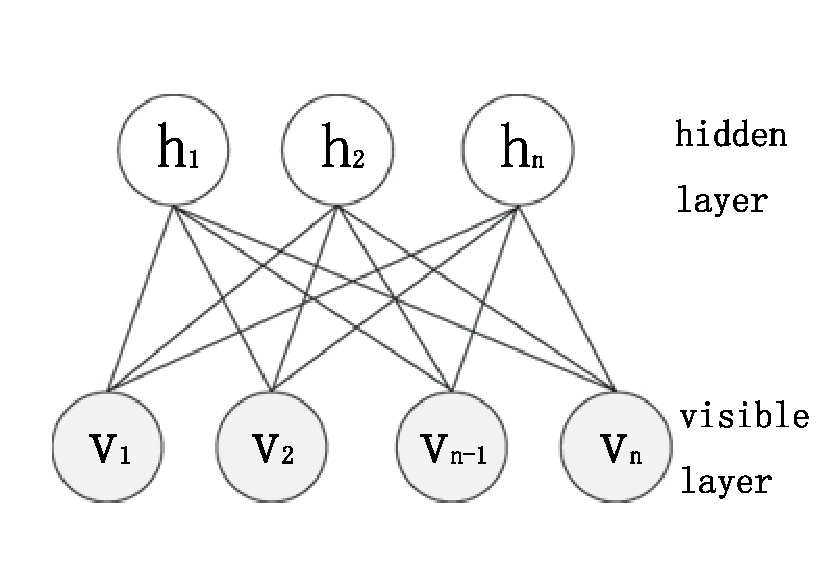
\includegraphics[width=2.5in]{rbm.eps}
\caption{A depiction of an two-layer RBM model, which included one layer with visible units and one layer with hidden units. Each visible unit is connected to the hidden units without visible-visible or hidden-hidden connections.}
\label{figure1}
\end{figure}

\subsubsection{Restricted Boltzmann machine}

Restricted Boltzmann Machine \cite{Ruslan} is a stochastic neural network with strong unsupervised learning ability. 
Figure \ref{figure1} depicted the RBM network structure.  
Each visible unit is connected to the hidden units without visible-visible or hidden-hidden connections. 
There were no connections between the visible and hidden layers.
The visible units were independent, then the Gibbs sampling method could be used to approximate the probability distribution. 
It consists of one layer of visible units with input $X = (v_1,v_2,...,v_n)$, one layer of hidden units with output $Y = (h_1,h_2,...,h_m)$ and two bias units whose states were always on and a way to adjusting the value of each unit. 

Boltzmann machine is based on statistical mechanics. The energy function $E(v,h)$ of an RBM was defined as:

\begin{equation}
E(v,h|\theta) = -\sum_{i=1}^n{a_iv_i}-\sum_{j=1}^m{b_ih_i}-\sum_{i=1}^n\sum_{j=1}^m{v_iW_{ij}h_j}
\end{equation}

$v$ and $h$ present the state vectors of the visible and hidden layers.$a_i$, $b_j$ and $W_{ij}$ are parameters, $\theta = \{W_{ij}, a_i, b_j\}$. So based on the energy function, the distribution of $v$ and $h$ is:

\begin{equation}
P(v,h|\theta) = \frac{e^{-E(v,h|\theta)}}{Z(\theta)}, Z(\theta) = \sum_{v,h}^{}{e^{-E(v,h|\theta)}}
\end{equation}

The purpose of RBM is to learn the optimal $\theta$. According to the probability distribution, the maximum likelihood function is defined as:

\begin{equation}
\theta^* = arg\max\limits_{\theta}L(\theta) = arg\max\limits_{\theta}\sum_{t=1}^T{\log P(v^{(t)}|\theta)}
\end{equation}
\begin{multline}
L(\theta) = \sum_{t=1}^T\Bigg (\log\sum_{h}^{}{exp[-E(v^{(t)},h|\theta)]}\\-\log\sum_{v}^{}{\sum_{h}^{}{[-E(v,h|\theta)]}}\Bigg)
\end{multline}
To get the optimal $\theta^*$, stochastic gradient descent\cite{Leon} method was used to maximum the likelihood function $L(\theta)$. The partial derivative of the parameters is shown below:

\begin{equation}
\begin{split}
&\frac{\partial\log P(v|\theta)}{\partial W_{ij}} = \langle v_i h_i \rangle_{data} -\langle v_i h_i \rangle_{model},\\
&\frac{\partial\log P(v|\theta)}{\partial a_{i}} = \langle v_i \rangle_{data} -\langle h_i \rangle_{model},\\
&\frac{\partial\log P(v|\theta)}{\partial b_{j}} = \langle h_i \rangle_{data} -\langle h_i \rangle_{model}.
\end{split}
\end{equation}
$\langle . \rangle_P$ denotes the distribution about P. $\langle . \rangle_{data}$ is easy to be calculated when the training samples were defined. $\langle . \rangle_{model}$ could not be resolved directly, but approximated by Gibbs sampling. Here we use the contrastive divergence(CD)\cite{Hinton02} algorithm proposed by Hinton in 2002, with which would achieve better results by only one step of Gibbs sampling .

\subsubsection{Softmax classifier}

This model generalized logistic regression \cite{Peng} in classification missions which would be useful in heartbeats arrhythmia classification problems. The softmax model is a kind of supervised learning method in conjunction with the deep belief network.

Supposing $m$ samples in the training set :
\begin{equation}
\{(x^{(1)},y^{(1)}), (x^{(2)},y^{(2)}), \ldots, (x^{(m)},y^{(m)}) \}
\end{equation}
the inputs were vectors $x^{(i)}$ corresponding to the features space. The labels are denoted by $y^{(i)}$  corresponding to the arrhythmia classes of the inputs.
The cost function of softmax regression with a weight decay term was defined as:

\begin{equation}
\begin{split}
J(\theta) = -\frac{1}{m}[\sum_{i=1}^m\sum_{j=1}^k1\{y^{(i)}=j\}\text{log}{\frac{e^{\theta_j^Tx^{(i)}}}{\sum_{l=1}^ke^{\theta_l^Tx^{(i)}}}}] \\
+ \frac{\lambda}{2} \sum_{i=1}^k \sum_{j=0}^n \theta_{jk}^2 (\lambda>0)
\end{split}
\end{equation}
and the partial derivative of the parameters were:
\begin{equation}
\begin{split}
\bigtriangledown_{\theta_j}J(\theta) = -\frac{1}{m}\sum_{i=1}^m[x^{(i)}(1\{y^{(i)}=j\}-p(y^{(i)}=j|x^{(i)};\theta))] \\
+ \lambda\theta_j  (\lambda>0)
\end{split}
\end{equation}
To train an optimum classifier, an optimization gradient descent algorithm called L-BFGS was used.

\begin{figure}[]
\centering
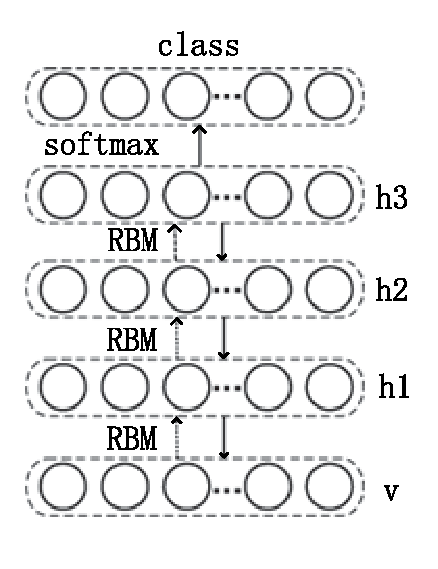
\includegraphics[width=2in]{dbn.eps}
% where an .eps filename suffix will be assumed under latex, 
% and a .pdf suffix will be assumed for pdflatex; or what has been declared
% via \DeclareGraphicsExtensions.
\caption{The RBMs are stacked to from a deep belief network(DBN). The RBM can be trained layer by layer. It is easy to construct a DBN with the trained RBMs. Also, a softmax model to fine-tune all parameters behind the last layer}
\label{figure2}
\end{figure} 

\subsubsection{Deep belief network}

Figure \ref{figure2} shows that RBMs can be stacked and trained with a greedy manner to form a deep belief network(DBN)\cite{Juergen, Bengio2009}. In the last layer, a softmax classifier is connected with the DBN. DBN is the graphical model of a hierarchical architecture. The five layers network shows in Figure\ref{figure2} are used to the heartbeat classification. The procedures were:
\begin{enumerate}
\item Train the first layer as an RBM which models the raw input $X$ as a visible layer.
\item After training the RBM, representations of the input were obtained.
\item Train the next layer as an RBM which models the transformed data as a visible layer.
\item Iterate step 2 and 3 for the desired number of layers.
\end{enumerate}

Finally the RBMs are combined to a DBN with the softmax model. Fine-tuning then was used as the supervised method to minimize the likelihood function and improve the adaptability. Here also the L-BFGS algorithm was used.

\subsection{Combined optimization algorithm for multi-lead classifiers}

The ECG wavelet transform performs differently in different channels by the waveforms. Each heartbeat channel shows diversely due to the P,QRS-complex and T wave constituent. 
Taking those into consideration, multi-lead ECG classification is significant improved by sample voting method. So a weight optimization method is proposed in two leads ECG signal classification. 
The method can be generally used in multi-lead ECG data classification. 

For each classifier trained with distinct lead, a reliability value is denoted as the accurate rate of the classifier. let $\gamma$ represent the reliability value. Then the classifiers' reliability is defined as $\gamma_1, \gamma_2, \cdots$

Using the testing samples to assess the result. The statistical matrix:
\begin{equation}
ClassSTST = \left(
\begin{array}{cccc}
 C_{11} & C_{12} & \cdots & C_{1n}\\
 C_{21} & C_{12} & \cdots & C_{2n}\\
 \cdots & \cdots & \ddots & \cdots\\
 C_{n1} & C_{n2} & \cdots & C_{nn}
\end{array}
\right)~
\end{equation}
In the statistical matrix, there are $n$ classes and $C_{11}$ represents the class \uppercase\expandafter{\romannumeral1} which is classified as class \uppercase\expandafter{\romannumeral1}, $C_{12}$ represents class \uppercase\expandafter{\romannumeral1} is classified as \uppercase\expandafter{\romannumeral2}, etc. 
The diagonal values are the correct classification. The purpose is to increase the diagonal values, so we adopt weights of the outputs for each classifier. 
The weights of the first classifier is $W_1 = (w_{11}, w_{12}, \cdots, w_{1n})$, the second were $W_2 = (w_{21}, w_{22}, \cdots, w_{2n})$. The constraint condition is $\sum\nolimits_{i=1}^2{w_{ik}} = 1$. 

First initial the weight to a mean value. Each sample has an output vector $O = {o_1, o_2, \cdots, o_n}$, the class is decided by the maximum value. Adding the weight of the value, the output is $(o_1w_1 ,o_2w_2, \cdots, o_nw_n)$. If the label of the sample is $l$, we would like to maximize $o_1w_{11} + o_1w_{21}$ while correspondingly minimize others. Through this, the $l$ class accurate is promoted while the false negative rate is also increased. The optimization algorithm would find a balance between the two weights of all testing samples. Accordingly, the optimal function is defined as :
\begin{equation}
F(x) = \frac{1}{\sqrt{2\pi}\sigma}x\exp^{-\frac{(x-\mu)^2}{2\sigma^2}}
\end{equation}
To find the maximum value of x, the derivative of the equation is:
\begin{equation}
\begin{split}
F^{'}(x) = 0, x = \frac{\mu}{2}+\sqrt{\frac{\mu^2}{4}+\sigma^2}
\end{split}
\end{equation}
Here, $\mu$ is denoted as initial weights. On the basis of the statistical matrix , counting the difference of the correct (diffcort) and false negative (diffflneg) quantities of the two classifiers. If the difference of the difference of the correct and false negative greater than zero, $\sigma^2 = \sqrt{\frac{diffcort - diffflsneg}{totalnumber}}$, so updating the corresponding class weight of the first classifier as $w_1 = \frac{\mu}{2}+\sqrt{\frac{\mu^2}{4}+\sigma^2}$. Else, $\sigma^2 = \sqrt{\frac{diffflsneg - diffcort}{totalnumber}}$, updating the weight of the second classifier as $w_2 = \frac{\mu}{2}+\sqrt{\frac{\mu^2}{4}+\sigma^2}$. Finally normalize the weights, the optimal combined value is $\gamma_1o_1w_1 + \gamma_2o_2w_2$. Generally, every two classifiers can be used to optimize the multi-lead ECG classification.

\subsection{ECG preprocessing}

The preprocessing works include two mainly parts, the ECG data filter and heartbeat segmentation process. The filter task is adapted to remove the artifact signal from the ECG signal. The artifact signal includes baseline wander, power line interference, and high-frequency noise. According to our pretraining works, the noise of the signal has little influence to the classifiers except for the baseline wander. So only baseline wander is removed. The massive unlabelled data we collected is extracted and a resample from 128Hz to 360Hz procedure is adopted for data consistency. In heartbeat segmentation process, average samples of each beat is 277 samples. To get more information , we allow partially overlap and a window with a length of 340 data points in one beat was defined, the R peak of the wave is located at 141th point. Most annotations of the MIT-BIH arrhythmia database is lied the R-wave. For the dataset we collect, a high accurate algorithm has been explored to determine the R pick and then divide into the heartbeat segments according to the R pick.

\subsection{RBM training}

The goal of RBM learning is to maximize the product of the probabilities. The parameters of the network can be initialized by the constructor. This option is useful when an RBM is used as the building block of the deep belief network, in which case the weight matrix and the hidden layer bias is shared with the corresponding layer of the network. The active function of the nodes is sigmoid function. The data is batched to train the RBM layer by layer. A single-step contrastive divergence(CD-1) is used in the gradient descent procedure. After calculating the partial derivative, the weights and bias is updated.


\begin{figure*}[t]
\centering
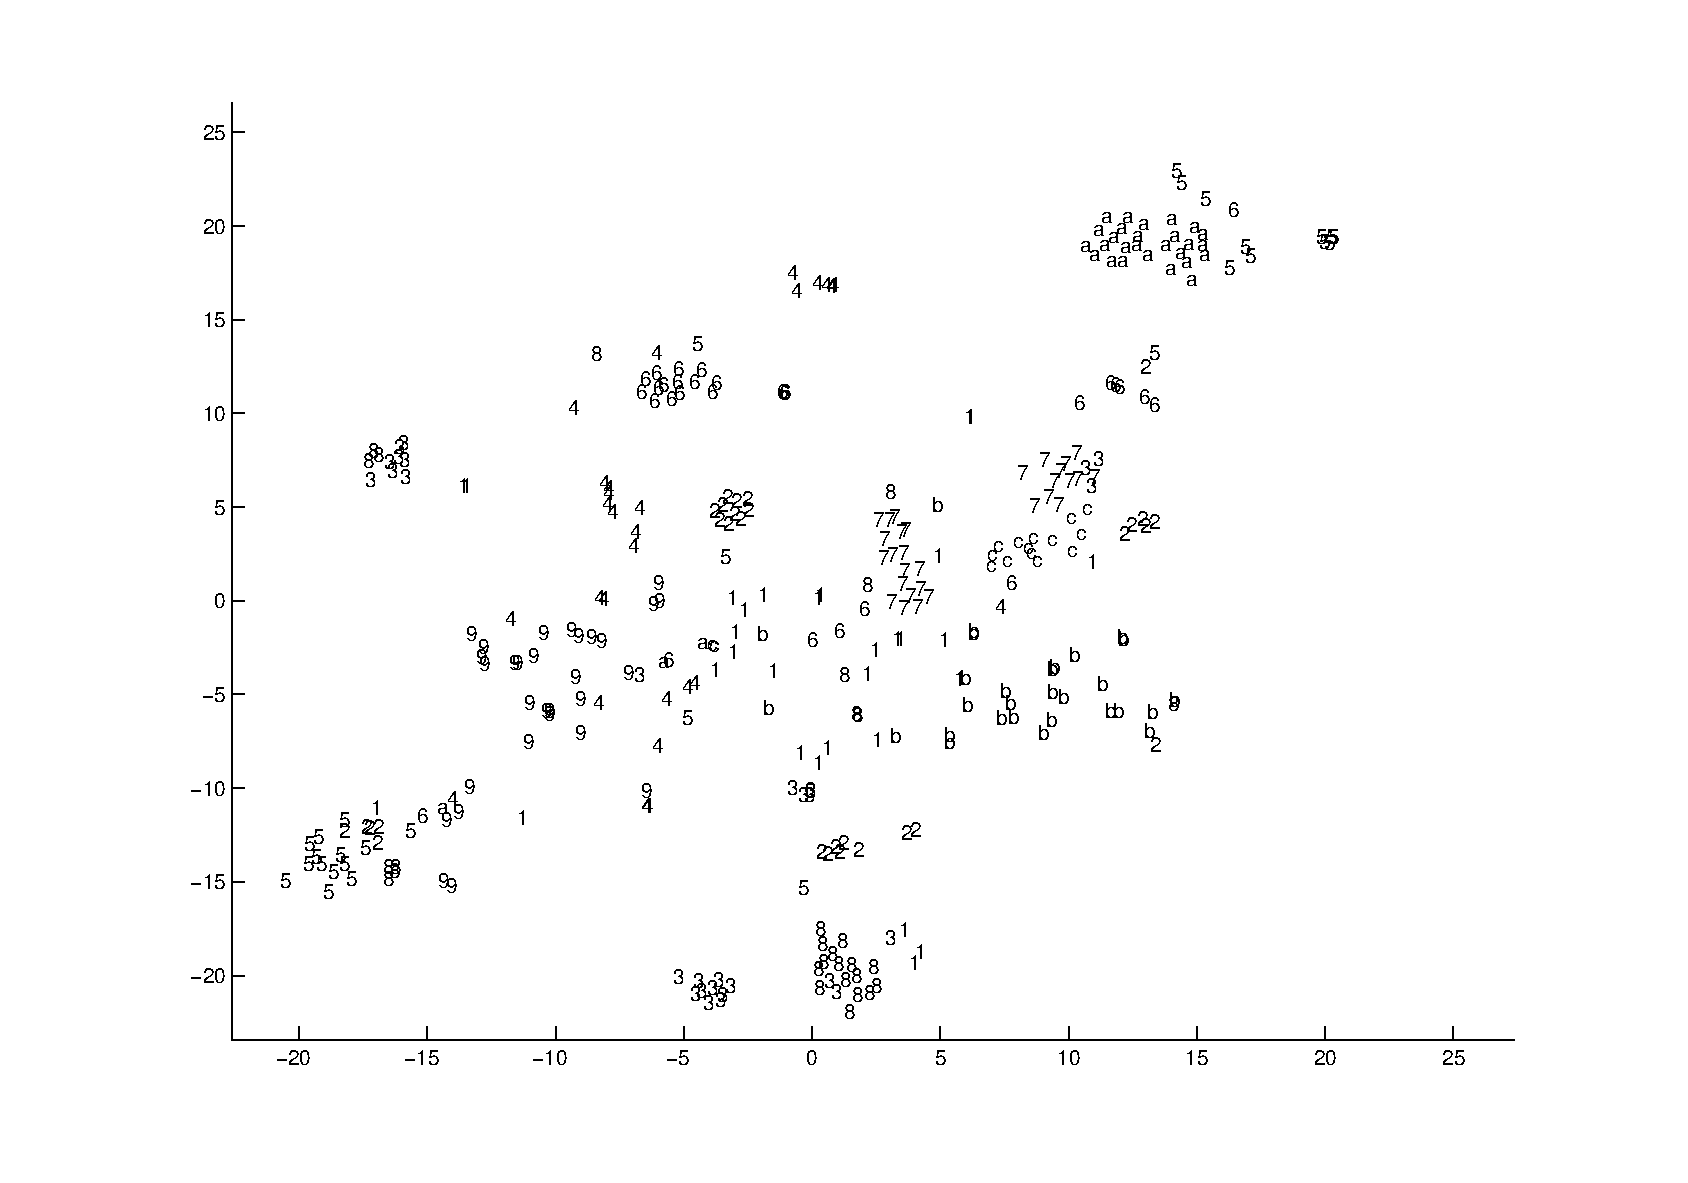
\includegraphics[width=7.2in]{distr.eps}
% where an .eps filename suffix will be assumed under latex, 
% and a .pdf suffix will be assumed for pdflatex; or what has been declared
% via \DeclareGraphicsExtensions.
\caption{The original heartbeats distribution visualizing with t-SNE \cite{Van}.}
\label{figure4}
\end{figure*}

\begin{figure*}[t]
\centering
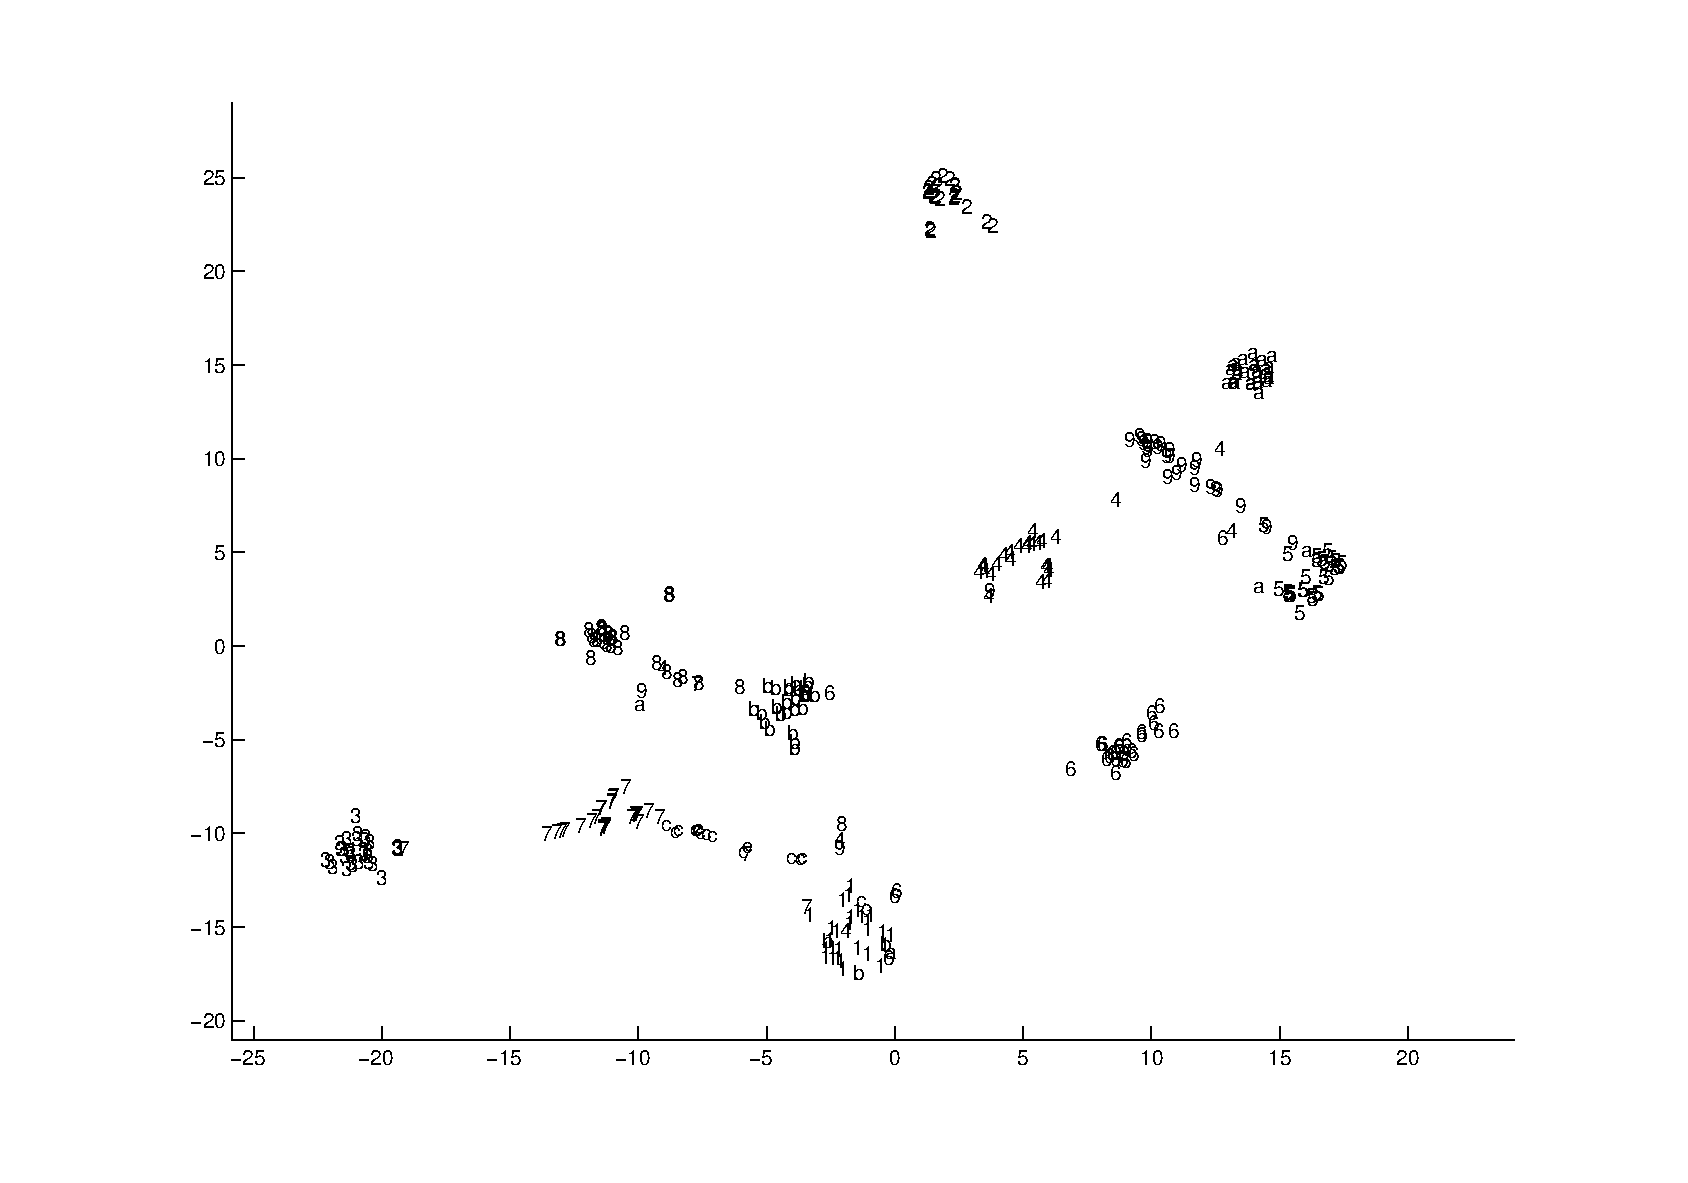
\includegraphics[width=7.2in]{mapdistr.eps}
% where an .eps filename suffix will be assumed under latex, 
% and a .pdf suffix will be assumed for pdflatex; or what has been declared
% via \DeclareGraphicsExtensions.
\caption{The output layer's corresponding heartbeats distribution visualized with t-SNE \cite{Van}.}
\label{figure5}
\end{figure*}

\subsection{DBN fine-tuning}

After the learning process, the RMBs can be used to initialize a deep belief network. Standard backpropagation algorithm can be applied to fine-tune the model. That can significantly improve the performance of the DBN. The fine-turning process is a supervised learning procedure, so at the last layer, a multi-class model called softmax is connected to classify the ECG data. Then using the fine-turning method to minimize the cost function.

\subsection{Performance assessment}

When finishing the fine-tuning process, the combining optimization algorithm was used to optimize the two-lead classifiers. The criterias employed to assess performance of beat classification approaches were sensitivity (TPR), specificity (SPC) and overall accuracy (ACC). Sensitivity is related to the correctly classified normal beats of normal beats
\begin{equation}
TPR = \frac{TP}{TP+FN}
\end{equation}
where TP(true positive) is the number of the correctly classified normal beats, FN(false negative) is the number of mistakenly classified normal beats. Specificity is the correctly classified abnormal beats
\begin{equation}
SPC = \frac{FN}{FP+TN}
\end{equation}
Where FP(false positive)is the number of the correctly classified abnormal beats, TN(true negative)is the number of the mistakenly classified corresponding abnormal beats Overall accuracy is the correctly classified beats
\begin{equation}
ACC = \frac{TP+TN}{TP+FP+NP+FN}
\end{equation}

\section{Experimental results}

In this section, the experimental results for the two leads ECG signal and combining algorithm are presented to evaluate the accuracy of the methods. The detail results are shown in Table \ref{table2}, \ref{table3} and \ref{table4}.

\begin{table*}[t]
\begin{center}
\begin{lrbox}{\tablebox}
\begin{threeparttable}
\caption{Test result of three hidden Layers deep belief network using first lead}
\label{table2}
\small
\begin{tabular}{cccccccccccccc}
\hline
\multicolumn{9}{r}{Algorithm classified label} \\
\cline{3-14}
		 &      & NORMAL & LBBB & RBBB & ABERR & PVC & FUSION & NPC & APC & FLWAV & VESC & NESC & AESC\\
\hline
 		 & NORMAL & 12,289& 3   &  2   &  3   &  15  &  9    &	0   &  37 &   2   &   0  &  0  &  0 \\
	     & LBBB   &  7    & 1,369&  0  &  0   &  6   &  0    &  0   &  1  &   0   &   0  &  0  &  0 \\
		 & RBBB   &  4    &  0  & 1,179&  0   &  3   &  0    &	0   &  4  &   0   &   0  &  0  &  0 \\
		 & ABERR  &  7    &  1  &  0   &  12  &  5   &  0    &	0   &  0  &   1   &   0  &  0  &  0 \\
		 & PVC    &  18   &  2  &  0   &  2   & 1,104&  8    &	0   &  2  &   2   &   0  &  0  &  0 \\
Original & FUSION &	 19   &  0  &  0   &  1   &  6   &   97  &	0   &  0  &   0   &   0  &  2  &  0 \\
label    & NPC    &	 5    &  0  &  1   &  0   &  0   &  0    &	4   &  1  &   0   &   0  &  1  &  0 \\
		 & APC    &	 58   &  2  &  9   &  0   &  2   &  0    &	0   &  382&   0   &   0  &  2  &  0 \\
		 & FLWAV  &	 10   &  0  &  0   &  1   &  8   &  0    &	0   &  0  &   58  &   0  &  0  &  0 \\
		 & VESC   &	 2    &  0  &  0   &  0   &  1   &  0    &	0   &  0  &   0   &  24  &  0  &  0 \\
		 & NESC   &	 6    &  0  &  1   &  0   &  0   &  0    &	0   &  1  &   0   &   0  &  15 &  0 \\
		 & AESC   &	 3    &  0  &  0   &  0   &  0   &  0    &	0   &  0  &   0   &   0  &  0  &  0 \\
\hline
\end{tabular}
\begin{tablenotes}
\item The test accuracy of the first lead is $98.247\%$.
\end{tablenotes}
\end{threeparttable}
\end{lrbox}
\scalebox{0.96}{\usebox{\tablebox}}
\end{center}
\end{table*}

\begin{table*}[!thbp]
\small
\begin{center}
\begin{lrbox}{\tablebox}
\begin{threeparttable}
\caption{Test result of three hidden layers deep belief network using second lead}
\label{table3}
\begin{tabular}{cccccccccccccc}
\hline
\multicolumn{9}{r}{Algorithm classified label} \\
\cline{3-14}
		 &      & NORMAL & LBBB & RBBB & ABERR & PVC & FUSION & NPC & APC & FLWAV & VESC & NESC & AESC\\
\hline
 		 & NORMAL & 12,233& 7   &  3   &  3   &  57  &  13   &	1   &  34 &   12  &   0  &  6  &  0 \\
	     & LBBB   &  12   & 1,366&  0  &  0   &  5   &  0    &  0   &  0  &   0   &   0  &  0  &  0 \\
		 & RBBB   &  5    &  0  & 1,169&  0   &  5   &  0    &	0   &  9  &   2   &   0  &  0  &  0 \\
		 & ABERR  &  7    &  0  &  1   &  10  &  6   &  0    &	1   &  0  &   1   &   0  &  0  &  0 \\
		 & PVC    &  56   &  3  &  1   &  0   & 1,048&  15   &	0   &  4  &   11  &   0  &  0  &  0 \\
Original & FUSION &	 22   &  0  &  0   &  0   &  5   &   97  &	0   &  0  &   0   &   0  &  1  &  0 \\
label    & NPC    &	 1    &  0  &  1   &  0   &  0   &  0    &	10  &  0  &   0   &   0  &  0  &  0 \\
		 & APC    &	 60   &  4  &  8   &  0   &  11  &  2    &	0   &  368&   1   &   0  &  0  &  1 \\
		 & FLWAV  &	 7    &  0  &  0   &  0   &  8   &  0    &	0   &  1  &   61  &   0  &  0  &  0 \\
		 & VESC   &	 2    &  0  &  1   &  0   &  2   &  0    &	0   &  0  &   2   &  20  &  0  &  0 \\
		 & NESC   &	 6    &  0  &  1   &  0   &  1   &  0    &	0   &  0  &   0   &   0  &  15 &  0 \\
		 & AESC   &	 2    &  0  &  0   &  0   &  0   &  0    &	0   &  0  &   0   &   0  &  0  &  1 \\
\hline
\end{tabular}
\begin{tablenotes}
\item The test accuracy of the second is $97.433\%$.
\end{tablenotes}
\end{threeparttable}
\end{lrbox}
\scalebox{0.96}{\usebox{\tablebox}}
\end{center}
\end{table*}

\begin{table*}[!htbp]
\small
\begin{center}
\begin{lrbox}{\tablebox}
\begin{threeparttable}
\caption{Test result of combination optimal algorithm with two leads}
\label{table4}
\begin{tabular}{cccccccccccccc}
\hline
\multicolumn{9}{r}{Algorithm classified label} \\
\cline{3-14}
		 &      & NORMAL & LBBB & RBBB & ABERR & PVC & FUSION & NPC & APC & FLWAV & VESC & NESC & AESC\\
\hline
 		 & NORMAL & 12,348& 0   &  0   &  0   &  11  &  2    &	0   &  7  &   1   &   0  &  0  &  0 \\
	     & LBBB   &  3    & 1,377&  0  &  0   &  3   &  0    &  0   &  0  &   0   &   0  &  0  &  0 \\
		 & RBBB   &  1    &  0  & 1,182&  0   &  2   &  0    &	0   &  5  &   0   &   0  &  0  &  0 \\
		 & ABERR  &  8    &  0  &  0   &  16  &  2   &  0    &	0   &  0  &   0   &   0  &  0  &  0 \\
		 & PVC    &  16   &  0  &  0   &  0   & 1,108&  10   &	0   &  1  &   3   &   0  &  0  &  0 \\
Original & FUSION &	 22   &  0  &  0   &  0   &  4   &   99  &	0   &  0  &   0   &   0  &  0  &  0 \\
label    & NPC    &	 3    &  0  &  0   &  0   &  0   &  0    &	9   &  0  &   0   &   0  &  0  &  0 \\
		 & APC    &	 58   &  2  &  5   &  0   &  1   &  0    &	0   &  389&   0   &   0  &  2  &  0 \\
		 & FLWAV  &	 2    &  0  &  0   &  0   &  6   &  0    &	0   &  0  &   69  &   0  &  0  &  0 \\
		 & VESC   &	 3    &  0  &  0   &  0   &  1   &  0    &	0   &  0  &   0   &  23  &  0  &  0 \\
		 & NESC   &	 11   &  0  &  1   &  0   &  0   &  0    &	0   &  1  &   0   &   0  &  11 &  0 \\
		 & AESC   &	 3    &  0  &  0   &  0   &  0   &  0    &	0   &  0  &   0   &   0  &  0  &  0 \\
\hline
\end{tabular}
\begin{tablenotes}
\item The test accuracy of the combining leads is $98.829\%$.
\end{tablenotes}
\end{threeparttable}
\end{lrbox}
\scalebox{0.96}{\usebox{\tablebox}}
\end{center}
\end{table*}

\subsection{The Segmentation of Heartbeat and Structure of DBN}

Each of the 44 records is slightly over 30 minutes long and 650000 samples. According to our count, each beat has about 277 samples. To get more information ,We allow part of overlap and define a window with length of 340 data points(the R peak of the wave is
located at 141th point). Considering the change of the heart rate, the window is adapted to avoid the mixture of two adjacent heart beats \cite{Burke}. The segmentation of the heartbeat depends on the R-peak detection, so a high precision algorithm based on the local maximum is used to detect the R peaks. The Mexican-Hat wavelet \cite{Burke} is also a choice to the R-peak detection.

The structure of the deep belief network we use is shown in Figure\ref{figure2}. The input layer is a vector of the heartbeat with 340 points and the nodes of hidden layer 1 is 200, hidden layer 2 is 200 and hidden layer 3 is 100. The output layer is a softmax model. The original ECG data is used to classify the heartbeat without features extraction process. Figure \ref{figure3} displays the error of the two channels using gradient descent algorithm when training the RBM. The t-SNE \cite{Van} algorithm is applied to visualize the distribution of heartbeat. 346 heartbeats are selected randomly from the dataset. It contains 30 heartbeats of each label from 1 to 11 and 16 heartbeats of all labeled 12 in the dataset. Figure \ref{figure3} clearly displays the distribution of the primal heartbeats. Figure \ref{figure4} shows the transformed features space. Character a represents label 10, b denotes label 11 and c indicates label 12. By comparing, the deep belief network is valid to heartbeats classification.

\begin{figure}[htb]
\centering
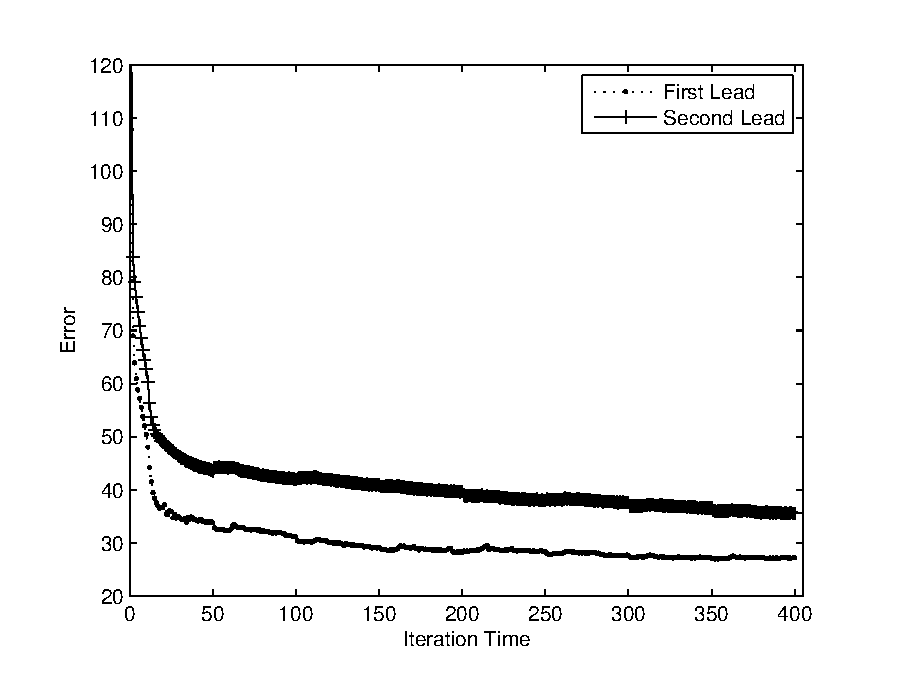
\includegraphics[width=3in]{error.eps}
% where an .eps filename suffix will be assumed under latex, 
% and a .pdf suffix will be assumed for pdflatex; or what has been declared
% via \DeclareGraphicsExtensions.
\caption{The cost of the two leads using gradient descent algorithm\cite{Leon} by RBM.}
\label{figure3}
\end{figure}

\subsection{The classification performance}

In the experiments, we adopted multi-lead ECG signal based on the restricted Boltzmann machine for the classification task. The MIT-BIH arrhythmia database is divided into three parts. Half of the beat is added to training the RBMs, one-third is applied to fine-tune the network and the left is used to test the model. In the 3 hidden layers deep belief network, the classifier outperforms in terms of sensitivity (SPR) $99.35\%$, specificity (SPC) $95.18\%$ and accuracy rate (ACC) $98.25\%$ using the first channels. Using the second channel we get the accuracy (ACC) of $97.43\%$, sensitivity (SPR) $98.90\%$ and specificity (SPC) $93.36\%$. At convergence of the optmization process, the combining method achieves the accuracy (ACC) of $98.83\%$, sensitivity (SPR) $99.83\%$ and specificity (SPC) $96.05\%$.

Table \ref{table2}, \ref{table3} and \ref{table4} illustrates the detail statistics information of the classifiers. The accurate rate is remarkably improved with the combining algorithm. It can be proved that multi-lead heartbeats classification is more reliable and higher in accuracy.

\section{Discussion}
One new aspect of this work is the new algorithm of combination in two ECG channels with deep belief network based on RBM. In previous study, most of the heartbeats classification used features extracted manually. In this research, the self learning method of heartbeat characteristics is illustrated. The detail performance is discussed below:

\subsection{Multilead fusion performance}
As the figures and tables in the experimental results showing, a better classification result had been achieved by the proposed method. Most of the accuracy of classes are improved by the combining algorithm in multi-lead signals.

For we use the limited labeled data from MIT database of only 51 persons, The network may be not fine-tuning to the best result state. As the classes statistics showed in Table \ref{table2}, \ref{table3} and \ref{table4}, the normal beats is very large, other's beat is less, so the most incorrect heartbeats are the abnormal beats classified to the normal. Properly augmenting the proportion of the abnormal heartbeats will significantly improve the accurate rate.

\subsection{The influence of filtering}

The artifact signal includes baseline wander, power line interference, and high-frequency noise. In this experiment, only the baseline wander is removed. According to our training progress, the power line interference and high-frequency noise has little effect on the deep belief network. From the testing result that we can state that the baseline removal filter affects the heartbeat classification in our proposed approach. The results confirm that the deep network works well on data with noisy. We adopt the same network structure and train all the classifiers with only baseline wander removed in the preprocessing progress. So the key difference between our work and others' is that we use simplex preprocessing and original ECG signal without complex features extraction.

\subsection{Compare with Others' works}

For we collect large amount of ECG data from the hospital which contains lots of normal beats and abnormal beats, the learning method of restricted Boltzmann machine is used to learning the features from the massive data by an unsupervised way. Then the RBMs is adapted to build a deep belief network. The optimization algorithm we propose improves the accuracy with multilead ECG signal. The heartbeat classification also has been studied by other algorithm, including hidden Markov model(HMM) \cite{Andreao}, support vector machine(SVM) \cite{Asl}\cite{Melgani}, independent component analysis(ICA) \cite{Sung}, Artificial neural networks(ANN) that use varied features extracted from the discreet signal data. Different performance assessment criteria has been adopted. In this comparison, we evaluate the performance on the indicators which put forward in the above sections: Sensitivity(TPR), specificity(SPC) and overall Accuracy(ACC). The $*NR$ symbol represents the result is not reported. 

\begin{table}[!htbp]
\small
\begin{center}
\begin{lrbox}{\tablebox}
\begin{threeparttable}
\caption{Comparisons with others' works}
\label{table5}
\begin{tabular}{lccc}
\hline

Approaches            	&  Accuracy(ACC)  & Sensitivity(TPR) & Specificity(SPC)\\
\hline
 Proposed             	&98.83\%   	  & 99.83\%  	 &96.05\%    \\
 Tadejko\cite{Tadejko}	& 97.82\%   	  & 99.70\%     &93.10\%    \\
 Banerjee\cite{Banerjee}&97.60\%  	  & 97.30\%     &98.80\%    \\
 Can\cite{Can}        	&99.71\%  	  & *NR         &*NR      \\
 Osowski\cite{Osowski}	&96.06\%   	  & 98.10\%     &95.53\%    \\
\hline
\end{tabular}
\begin{tablenotes}
\item [a] *NR means the results were not reported.
\item [b] The listed percentages are based on the assessment rules.
\end{tablenotes}
\end{threeparttable}
\end{lrbox}
\scalebox{0.92}{\usebox{\tablebox}}
\end{center}
\end{table}

The Table \ref{table5} shows the performance of different models that used for the heartbeat classification, the proposed method offers a high accuracy of classification. 

All the annotations in the MIT-BIH arrhythmia database is use in our study and Osowski\cite{Osowski} only selects 7 types. Can\cite{Can} get the highest accuracy but with a
price of rejecting 2054 heartbeats(2.4\% rejections). By comparing with others' experience, our approach provided higher performance in heartbeat classification without complex wavelet transform algorithms. 


\section{Conclusions}

This study shows that how a restricted Boltzmann machine works with large scale of ECG data.  Training a deep belief network is time-consuming job, but it works fast to predict. Using the MIT-BIH Arrhythmia Database \cite{Goldberger} and massive data we collected from the hospital, the batch progressing method is applied to speed up the training progress. At last, a fine-tuning method is used to adapt the whole network. From the obtained experimental results, it can be strongly recommended that the deep belief network is suitable to ECG classification. We test 16,831 samples randomly chosen from MIT-BIH and provide them with high accuracy of $98.247\%$ from the first channel ECG signal and $97.433\%$ from the second channel. By learning features from massive data the model can get a more accurate result. Another advantage of the multi-lead RBMs training progress can be found in its parallel. The training of different channel does not affect each other. So this method enhance the classification accuracy and does not increase the training time.

An optimization method is proposed for multi-lead heartbeat classification. The system shows better result with this method. Also the method is acting on the output of the deep belief network. The combined result is $98.829\%$ in two channels which is better than with only one channel. For different channel shows diverse degrees of the components, the result confirmed that optimal algorithm substantially boosts the accuracy of the heartbeat classification with multi-lead. From the filtering process, the deep belief network is well robust with the original data has noise. 

\section*{Acknowledgment}
This study was financed partially by the National 863 Program of China (Grant No. 2012AA02A604), the Next generation communication technology Major project of National S\&T (Grant No. 2013ZX03005013), the Key Research Program of the Chinese Academy of Sciences, and the Guangdong Innovation Research Team Funds for Image-Guided Therapy and Low-cost Healthcare. 
% trigger a \newpage just before the given reference
% number - used to balance the columns on the last page
% adjust value as needed - may need to be readjusted if
% the document is modified later
%\IEEEtriggeratref{8}
% The "triggered" command can be changed if desired:
%\IEEEtriggercmd{\enlargethispage{-5in}}

% references section

% can use a bibliography generated by BibTeX as a .bbl file
% BibTeX documentation can be easily obtained at:
% http://www.ctan.org/tex-archive/biblio/bibtex/contrib/doc/
% The IEEEtran BibTeX style support page is at:
% http://www.michaelshell.org/tex/ieeetran/bibtex/
%\bibliographystyle{IEEEtran}
% argument is your BibTeX string definitions and bibliography database(s)
%\bibliography{IEEEabrv,../bib/paper}
%
\bibliographystyle{IEEEtran} % Style BST file
\bibliography{RBM}  
% <OR> manually copy in the resultant .bbl file
% set second argument of \begin to the number of references
% (used to reserve space for the reference number labels box)
%\begin{thebibliography}{2}

%\bibitem{tanis}
%T.~Mar, S.~Zaunseder, J.P.~Martinez, M.~Llamedo and R.~Poll, \emph{Optimization of electrocardiography Classification by Means of Feature Selection}.\hskip 1em plus
%  0.5em minus 0.4em\relax Harlow, England: Addison-Wesley, 1999.
  
%\bibitem{care}
%H.~Kopka and P.~W. Daly, \emph{A Guide to \LaTeX}, 3rd~ed.\hskip 1em plus
%  0.5em minus 0.4em\relax Harlow, England: Addison-Wesley, 1999.
  
%\end{thebibliography}

% biography section
% 
% If you have an EPS/PDF photo (graphicx package needed) extra braces are
% needed around the contents of the optional argument to biography to prevent
% the LaTeX parser from getting confused when it sees the complicated
% \includegraphics command within an optional argument. (You could create
% your own custom macro containing the \includegraphics command to make things
% simpler here.)
%\begin{IEEEbiography}[{\includegraphics[width=1in,height=1.25in,clip,keepaspectratio]{mshell}}]{Michael Shell}
% or if you just want to reserve a space for a photo:

\begin{IEEEbiography}{Jan Doe}
Biography text here.
\end{IEEEbiography}
% if you will not have a photo at all:
\begin{IEEEbiographynophoto}{John Doe}
Biography text here.
\end{IEEEbiographynophoto}

% insert where needed to balance the two columns on the last page with
% biographies
%\newpage

\begin{IEEEbiographynophoto}{Jane Doe}
Biography text here.
\end{IEEEbiographynophoto}

% You can push biographies down or up by placing
% a \vfill before or after them. The appropriate
% use of \vfill depends on what kind of text is
% on the last page and whether or not the columns
% are being equalized.

%\vfill

% Can be used to pull up biographies so that the bottom of the last one
% is flush with the other column.
%\enlargethispage{-5in}

% that's all folks
\end{document}


